\documentclass[12pt,aspectratio=169, colorlinks=true, linkcolor=circlBlue]{beamer}

% tlp allowed values: clear, green, amber, amber+strict, red
\usetheme[numbering=fraction, progressbar=frametitle]{circl}

% for code highlighting
\usepackage{minted}
% to draw pingus
\usepackage{tikzpingus}
% to draw boxes to catch attention
\usepackage{awesomebox}
% For hyperlinks in the document and PDF metadata
\usepackage{hyperref}
% useful only if we want to customize minted background
\usepackage{tcolorbox}

\definecolor{monokaiBackground}{rgb}{0.15, 0.15, 0.15}
% if this is defined globally it will apply to all minted boxes
\tcolorboxenvironment{minted}{
    %colback=monokaiBackground, % Use the defined color here
    boxrule=0pt,               % Remove border
    arc=5pt, % Rounded borders
    left=2pt, right=2pt, top=2pt, bottom=2pt % Margins
}

\hypersetup{
    pdftitle={Presentation title},    % Title
    pdfauthor={Firstname Lastname},               % Author
    pdfsubject={Brief description}, % Subject
    pdfkeywords={tag1, tag2, tag3}, % Keywords
    colorlinks=false,                       % Color links instead of boxes
    linkcolor=blue,                        % Color of internal links
    citecolor=blue,                        % Color of citations
    urlcolor=blue                          % Color of external links
}

% set the logo to put in the title page
\titlegraphic{\noindent\hfill
\includegraphics[width=0.3\textwidth]{img/logo-circl.pdf}}
\title{Introduction to endpoint visibility}
%\subtitle{An Open-Source Threat-Detection Tool for Linux}
\date{2025/05/26}
\author{Quentin JEROME (quentin.jerome@circl.lu)}
\institute{University of Luxembourg - Luxembourg}
% if set inserts a title link into the title page
%\titlelink{\faGithub\space \normalurl{https://github.com/CIRCL/website}}

\begin{document}

% include custom commands

% Place here your custom commands, it will be included in presentation.tex

\newcommand{\normalurl}[1]{\href{#1}{#1}}

\newcommand{\footnoteurl}[1]{\footnote{\scriptsize\url{#1}}}

\newcommand{\rocketbox}[1]{%
	\awesomebox[circlRed]{1pt}{\faRocket}{circlBlue}{#1}%
}

% Title page
\begin{frame}
	\titlepage%
\end{frame}

\begin{frame}{Question?}
	\begin{center}
		\Huge Do you have an idea\\
		how antivirus software works?
	\end{center}
\end{frame}

\begin{frame}{How Antivirus Works}
	\begin{itemize}
		\item Antivirus software primarily uses signature-based detection:
		      \begin{itemize}
			      \item Scans files and processes for known malware signatures
			      \item Relies on databases regularly updated with new threat signatures
		      \end{itemize}
		\item Some AVs use heuristic or behavior-based detection to catch unknown threats
		\item However, advanced threats often evade detection by:
		      \begin{itemize}
			      \item Using custom or polymorphic malware
			      \item Employing stealth techniques and zero-day exploits
		      \end{itemize}
	\end{itemize}
\end{frame}

\begin{frame}{Antivirus Management in Large Organizations}
	\begin{itemize}
		\item Antivirus software is just another IT tool to deploy and maintain
		\item Often managed by software or IT teams, not specialized security teams
		\item Limited involvement of security experts in configuring or responding to alerts
		\item AV alerts often handled as routine IT issues rather than security incidents
	\end{itemize}
\end{frame}

\begin{frame}{Question?}
	\begin{center}
		\Huge Is the traditional antivirus model\\
		effective at detecting\\
		advanced targeted threats?
	\end{center}
\end{frame}

\begin{frame}{Not Really!}
	\begin{itemize}
		\item Traditional antivirus relies mostly on known signatures (static and dynamic)
		\item Advanced targeted threats use custom malware, polymorphic code, unknown techniques and sometimes zero-days
		\item Such threats often evade signature-based detection (because they have tested their malware against the AV the targeted entity is running)
		\item Heuristic and behavior-based methods improve detection but have limits
	\end{itemize}
\end{frame}

\begin{frame}{Limitations of AV Software}

	(Ideally) they have to \textbf{detect} all malware and they have \textbf{not to detect}
	all benign software, this in a single product distributed to all customers!

	\begin{itemize}
		\item What is a malware?
		\item Does everyone have the same definition?
	\end{itemize}

	\awesomebox[circlRed]{2pt}{\faLightbulb}{circlBlue}{
		\large{AV impose to their definition of what is a malware and what is not. While providing no context about their detections.}
	}
\end{frame}

\begin{frame}{Question?}
	\begin{center}
		\Huge What is the main objective when doing incident response?
	\end{center}
\end{frame}

\begin{frame}{What Are We Trying to Achieve in Incident Response?}
	\begin{itemize}
		\item The main objective: \textbf{gather context around an alert} to understand the incident
		\item Context includes:
		      \begin{itemize}
			      \item What triggered the alert?
			      \item What happened before and after?
			      \item Which users, processes, and systems were involved?
		      \end{itemize}
		\item This contextual information is essential to:
		      \begin{itemize}
			      \item Assess the impact and scope of the incident
			      \item Build and update the \textbf{incident timeline}
			      \item Guide response actions and recovery
		      \end{itemize}
	\end{itemize}

\end{frame}



\begin{frame}{Incident Response Mantra}
	\faLightbulb \centering\large\textbf{ Without context, alerts are just noise.}
	\begin{itemize}
		\item An alert alone tells you something happened — but not what, why, or how.
		\item Context transforms a raw signal into actionable intelligence:
		      \begin{itemize}
			      \item Who did it?
			      \item What else happened around the same time?
			      \item Is it part of a larger pattern?
		      \end{itemize}
		\item Effective incident response is not just reacting to alerts — it's \textbf{investigating with context}.
	\end{itemize}
\end{frame}

\begin{frame}{Question?}
	\begin{center}
		\Huge Knowing that, how do you think\\
		incident response goes with AV alerts only?
	\end{center}
\end{frame}

\begin{frame}{Bad}
	\begin{itemize}
		\item Limited visibility into what actually happened during an attack
		\item Difficulty in tracing attack vectors and lateral movements
		\item Delays in detection reduce chances for quick containment
		\item Lack of rich context makes investigations slow and inefficient
	\end{itemize}

	\awesomebox[circlRed]{2pt}{\faLightbulb}{circlBlue}{
		\large{Security teams need transparent, flexible, and extensible tools to monitor endpoints \textrightarrow \textbf{endpoint visibility software}}
	}
\end{frame}

\begin{frame}{What is an Endpoint Visibility Software?}
	A tool that monitors and collects information from endpoints (servers, workstations, network devices)
	\begin{itemize}
		\item Provides real-time insights into what is happening on a system:
		      \begin{itemize}
			      \item Process executions
			      \item File accesses and modifications
			      \item User activities
			      \item Network connections
		      \end{itemize}
		\item Helps detect suspicious or malicious behaviors
		\item Essential to implement \textbf{customized / tailored} threat detection scenarios
	\end{itemize}
\end{frame}

\begin{frame}{Beyond Detection: Incident Response Value}
	Endpoint visibility tools are not only useful for threat detection
	\begin{itemize}
		\item They provide \textbf{invaluable data} during incident response:
		      \begin{itemize}
			      \item Timeline reconstruction of attacker activity
			      \item Identification of persistence mechanisms
			      \item Tracing lateral movement across systems
			      \item Understanding the scope and impact of the breach
		      \end{itemize}
		\item Without visibility, responders are often blind, forced to make assumptions while relying on time consuming analysis methods
		      \begin{itemize}
			      \item Quick artifact acquisition (\texttt{osquery}, \texttt{velociraptor})
			      \item Disk acquisition (need someone with a physical access to the device)
			      \item Artifact / disk acquisition take time and any time saved in incident response is good to take
		      \end{itemize}
	\end{itemize}
\end{frame}

\begin{frame}
	\frametitle{Specific Terminology}
	\begin{itemize}
		\item \textbf{Security event}: an event happening on a system which may indicate a potential security incident
		      \begin{itemize}
			      \item[] \textbf{Example}: A log entry that indicates the execution of a given binary
		      \end{itemize}

		\item \textbf{Security monitoring tool}: a tool monitoring a system or an infrastructure and generating security events for analysis.
		      \begin{itemize}
			      \item[] \textbf{Example}: Intrusion Detection Systems (IDS), Endpoint Detection and Response (EDR)
		      \end{itemize}

		\item \textbf{Security visibility}: the ability to monitor,detect and analyze security events
		      \begin{itemize}
			      \item[] \textbf{Example}: A company using a security monitoring software increases its security visibility
		      \end{itemize}

	\end{itemize}
\end{frame}

\begin{frame}
	\frametitle{Different Software for Different Purposes}
	\begin{center}
		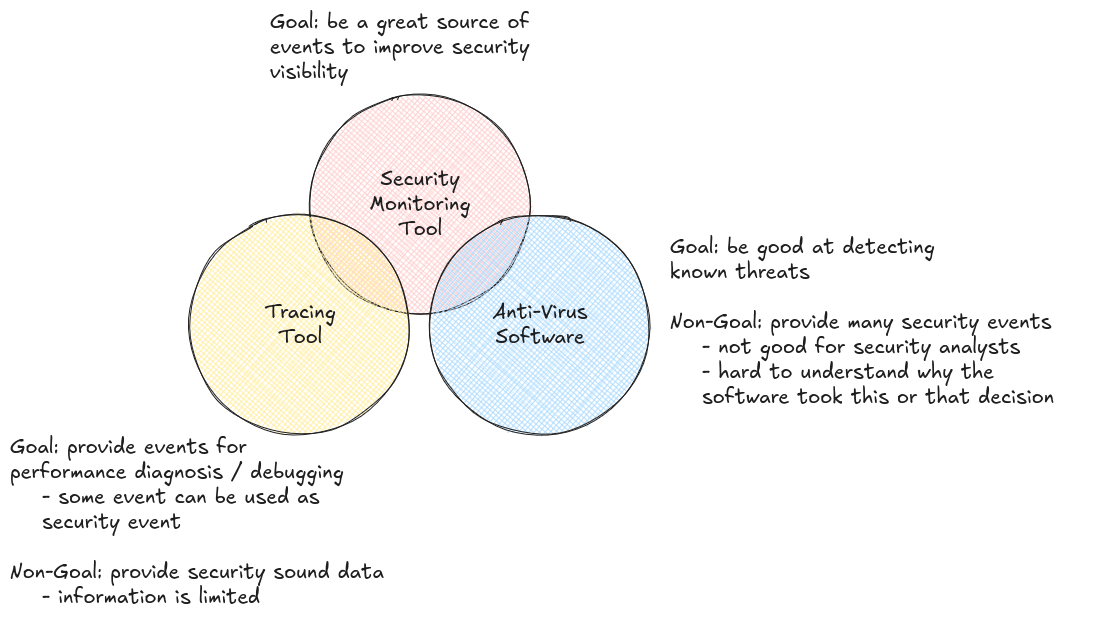
\includegraphics[width=0.9\textwidth]{img/different-tools.png}
	\end{center}
\end{frame}

\begin{frame}{Question}
	\begin{center}
		\Huge{Do you know any endpoint visibility software?}
	\end{center}
\end{frame}

\begin{frame}{Current Landscape of Endpoint Visibility Software}
	\begin{itemize}
		\item Real-time visibility is essential for detecting and responding to threats
		\item Few open-source tools provide comprehensive real-time event collection
		\item \textbf{Linux:}
		      \begin{itemize}
			      \item \texttt{Auditd} – Kernel-level auditing, powerful but complex
			      \item \texttt{Kunai} – Real-time system event collection and threat hunting
			      \item \texttt{Falco} – Real-time detection focused on containers and syscall activity
		      \end{itemize}
		\item \textbf{Windows:}
		      \begin{itemize}
			      \item \texttt{Sysmon} – Free tool from Microsoft for detailed event logging (not open-source)
			      \item \texttt{Wazuh} – Some real-time monitoring via event/log analysis
		      \end{itemize}
	\end{itemize}
\end{frame}

\begin{frame}{Key Steps for Effective Endpoint Visibility (1/2)}
	\begin{enumerate}
		\item \textbf{Monitor Endpoints}
		      \begin{itemize}
			      \item Deploy lightweight agents or kernel features to collect real-time events
		      \end{itemize}

		\item \textbf{Define Logging Policies}
		      \begin{itemize}
			      \item Determine what events are relevant (processes, file changes, network activity)
			      \item Balance between data volume and usefulness
		      \end{itemize}

		\item \textbf{Forward and Aggregate Logs}
		      \begin{itemize}
			      \item Securely send logs to central servers or SIEM platforms
			      \item Ensure reliability and scalability
		      \end{itemize}
	\end{enumerate}
\end{frame}

\begin{frame}{Key Steps for Effective Endpoint Visibility (2/2)}
	\begin{enumerate}
		\setcounter{enumi}{3}
		\item \textbf{Analyze and Correlate}
		      \begin{itemize}
			      \item Use rules, heuristics, and behavioral analytics to detect anomalies
			      \item Enrich events with contextual data for better investigations
		      \end{itemize}

		\item \textbf{Respond and Hunt}
		      \begin{itemize}
			      \item Trigger alerts, perform threat hunting, and conduct incident response
			      \item Continuously refine detection and response strategies
		      \end{itemize}
	\end{enumerate}
\end{frame}

\begin{frame}{With Great Power Comes Great Responsibilities (1/2)}
	\begin{itemize}
		\item \textbf{1. Choosing the right data:}
		      \begin{itemize}
			      \item Select logs that are useful for detection
			      \item Select logs that support incident response and forensics
		      \end{itemize}
		\item \textbf{2. Performance considerations:}
		      \begin{itemize}
			      \item Minimize CPU, memory, and disk impact on monitored endpoints
			      \item Ensure tools do not degrade system reliability
		      \end{itemize}
		\item \textbf{3. Backend pressure:}
		      \begin{itemize}
			      \item Limit log volume to avoid overloading storage and processing pipelines
			      \item Enable long-term retention with reasonable storage costs
		      \end{itemize}
	\end{itemize}
\end{frame}

\begin{frame}{With Great Power Comes Great Responsibilities (2/2)}
	\begin{itemize}
		\item \textbf{4. Signal-to-noise ratio:}
		      \begin{itemize}
			      \item Avoid collecting redundant or low-value events
			      \item Prioritize actionable and context-rich logs
		      \end{itemize}
		\item \textbf{5. Security and privacy:}
		      \begin{itemize}
			      \item Protect collected data (it may contain sensitive information)
			      \item Comply with legal and organizational data retention policies
		      \end{itemize}
	\end{itemize}


	\awesomebox[circlRed]{2pt}{\faLightbulb}{circlBlue}{
		\large{\textbf{Analyst / detection engineers} will want all the logs possible but you will have to do \textbf{trade-offs}}
	}

\end{frame}


\begin{frame}{Theory vs. Practice in Endpoint Visibility}
	In theory, comprehensive endpoint monitoring covers all systems and activities
	\begin{itemize}
		\item In practice, blind spots remain due to:
		      \begin{itemize}
			      \item Legacy systems running critical but unmodifiable applications
			      \item Network appliances and proprietary hardware with limited visibility
			      \item Constraints on deploying agents or updating software
		      \end{itemize}
		\item These gaps require tailored solutions and additional network-level monitoring
	\end{itemize}

	\awesomebox[circlRed]{2pt}{\faLightbulb}{circlBlue}{
		\large{Endpoint visibility is necessary but not always sufficient for full coverage}
	}
\end{frame}

\begin{frame}{Question}
	\begin{center}
		\Huge Do you believe we should\\
		throw antivirus away?
	\end{center}
\end{frame}

\begin{frame}{Of Course Not}
	\begin{itemize}
		\item Antivirus can still serve as a first layer of defense
		\item Antivirus have very solid signature database detecting many commodity malware you don't want to bother with
		\item It might detect some threats or serve as a trigger for deeper investigations
		\item AV should be used \textbf{in conjunction with} a solid endpoint visibility strategy
	\end{itemize}

	\awesomebox[circlRed]{2pt}{\faRocket}{circlBlue}{
		\large{Combining AV software with a good endpoint visibility strategy improves detection rates and shortens incident response time}
	}
\end{frame}

\begin{frame}{Key Takeaways}
	\begin{itemize}
		\item \textbf{Traditional antivirus} mainly detects known threats using signatures — often ineffective against advanced attacks.
		\item \textbf{AV alerts lack context}, making incident response difficult and slow.
		\item \textbf{Context is king}: effective incident response requires understanding what happened before, during, and after an alert.
		\item \textbf{Endpoint visibility tools} provide real-time, high-context data critical for detection and response.
		\item \textbf{With great power comes responsibility}: collecting the right logs, minimizing system impact, and balancing retention and privacy are essential.
		\item \textbf{AV is not obsolete} — it still plays a role as part of a layered security approach.
	\end{itemize}
\end{frame}


\section{Linux Endpoint Visibility with Kunai}

\begin{frame}{What is Kunai?}
	\textbf{Kunai} is a free and open-source Linux endpoint monitoring and hunting tool
	\begin{itemize}
		\item Designed to provide deep visibility into what happens on a Linux system
		\item Features:
		      \begin{itemize}
			      \item Lightweight agent for collecting real-time system events
			      \item Extensible rule engine for detecting suspicious or malicious activity
			      \item Outputs structured \texttt{JSON} events for easy integration and analysis
			      \item Correlates with tools like \textbf{Suricata} and \textbf{Zeek} for enriched detection
		      \end{itemize}
		\item Aimed at individuals, companies, and public sector entities looking to improve visibility and response
	\end{itemize}
\end{frame}

\begin{frame}{But, why Kunai?}
	\awesomebox[circlRed]{2pt}{\faRocket}{circlBlue}{
		\large{Kunai is \textbf{open-source} and is developed here in \textbf{Luxembourg}}
	}

	\centering{\textbf{Many concepts} you will learn with Kunai will be transposable into other tools}
\end{frame}

\begin{frame}{Q\&A}
	\centering\huge{Any question?}
\end{frame}

\begin{frame}{Exercises}
	\centering\url{https://hdoc.csirt-tooling.org/5VEw-vd_ShmRs0T0307lSQ\#}
\end{frame}

\end{document}
